\section*{Results}

% In the Results section, you should demonstrate your baseline model’s performance, perfor- mances for each of the parts of Q4.b and Q4.c. You should include both of the performance metrics described in Evaluation metrics (see part 1 above in Implementation Instructions). Please organize these results into a series of concise tables. The formatting is your choice, as long as it is easily interpretable.
% For each architecture include:
% (a) A single plot showing both training and validation loss curves;
% (b) Validation set pixel accuracy and average IoU.
% (c) Visualizations of the segmented output for any one image in the test set along with the original image. Use the color coding mapping in the voc.py for this (Please refer to visualize.ipynb for help on plotting).

\subsection*{Baseline FCN}

On the validation set, the baseline had an average IOU of 0.08 and 77\% pixel accuracy. Our baseline FCN resulted in a 0.06 IOU and a 75\% pixel accuracy on the test set.

\begin{figure}[H]
	\centering
	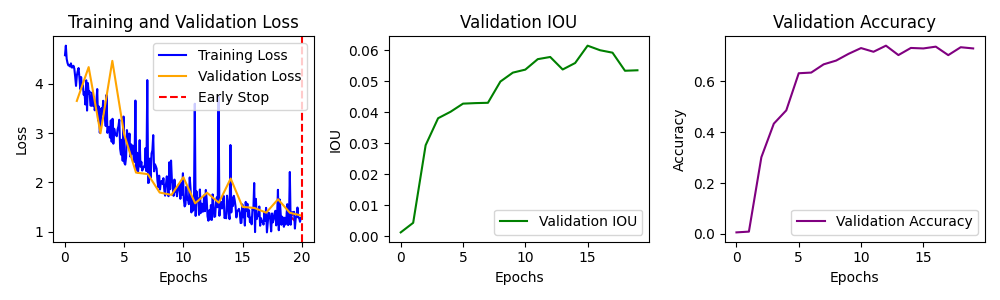
\includegraphics[width=\textwidth]{plots/baseline}
	\caption{Baseline Augmentation}
	\label{fig:baseline}
\end{figure}

\subsection*{FCN with augmentation}

The average IOU and pixel accuracy for the validation set were 0.07 and 74\%. Our FCN with augmentation resulted in a 0.06 IOU and a 72\% pixel accuracy on the test set. We noticed that the loss convergence
was slower.

\begin{figure}[H]
	\centering
	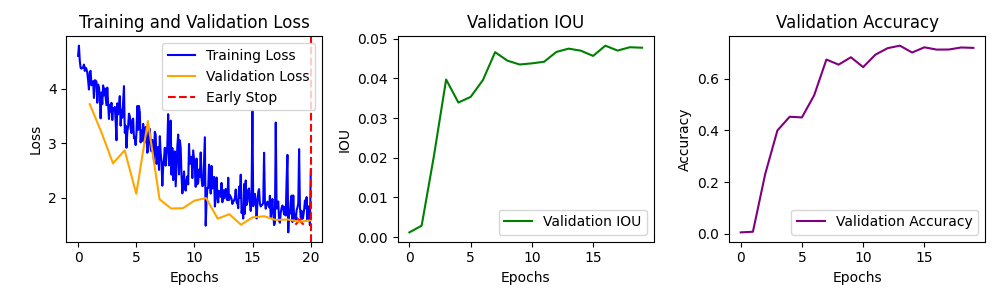
\includegraphics[width=\textwidth]{plots/baseline_augmentation}
	\caption{Baseline Augmentation}
	\label{fig:baseline_aug}
\end{figure}

\subsection*{FCN with Cosine Annealing LR}

The validation set resulted in an average IOU of 0.06 and a pixel accuracy of 75\%. Our FCN with Cosine Annealing LR resulted in a 0.05 IOU and a 74\% pixel accuracy on the test set.


\begin{figure}[H]
	\centering
	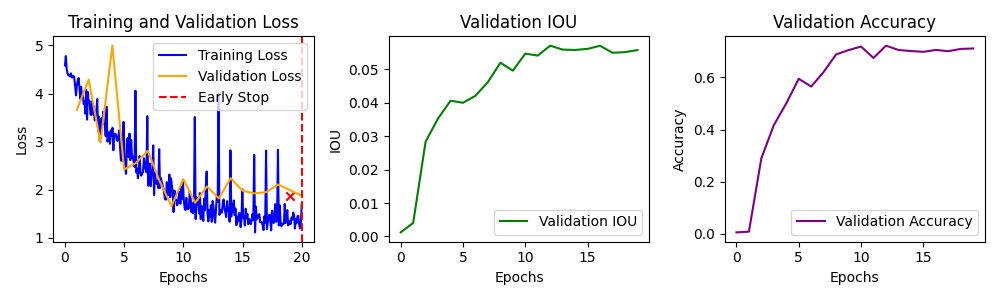
\includegraphics[width=\textwidth]{plots/baseline_cosine}
	\caption{Baseline Cosine}
	\label{fig:baseline_cos}
\end{figure}

\subsection*{FCN with Custom Class Weights}


From the validation set, the average IOU and pixel accuracy were 0.05 and 69\%. Our FCN with custom class weights resulted in a slightly worse 0.04 IOU and a 67\% pixel accuracy on the test set.

\begin{figure}[H]
	\centering
	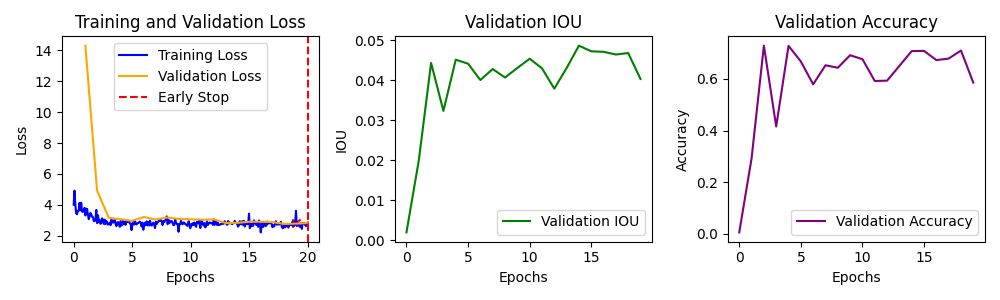
\includegraphics[width=\textwidth]{plots/baseline_weights}
	\caption{Baseline Weights}
	\label{fig:baseline_weights}
\end{figure}

\subsection*{DarrenNet}

In Figure \ref{fig:darren}, we observe the outcomes of DarrenNet. Validation set results were an IOU of 0.07 and a pixel accuracy of 77\% The model has a respectable IOU (0.05) and accuracy (75\%), while maintaining very fast training speeds.

\begin{figure}[H]
	\centering
	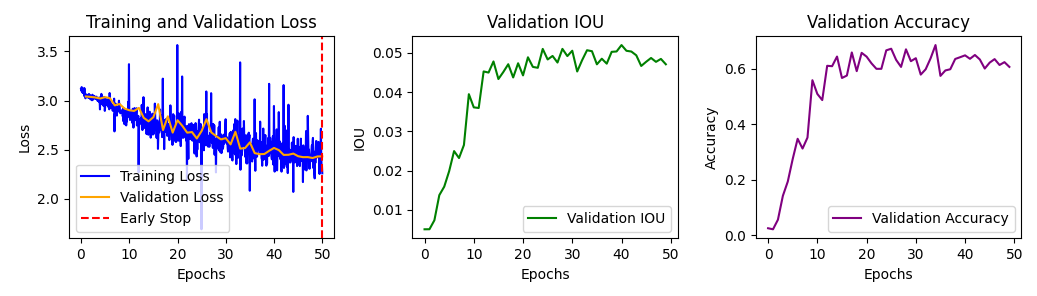
\includegraphics[width=\textwidth]{plots/darrennet}
	\caption{DarrenNet}
	\label{fig:darren}
\end{figure}


In Figure \ref{fig:darren_transfer}, we observe the outcomes of DarrenNet with transfer learning using resnet34's encoder. The model leverages pre-trained weights, demonstrating superior performance on the test set. The average IOU and pixel accuracy for the validation set were 0.12 and 78\%. The transfer learning strategy significantly boosts both IOU (0.10) and accuracy (78\%), indicating that the network effectively transfers knowledge from the source domain to the target domain.


\begin{figure}[H]
	\centering
	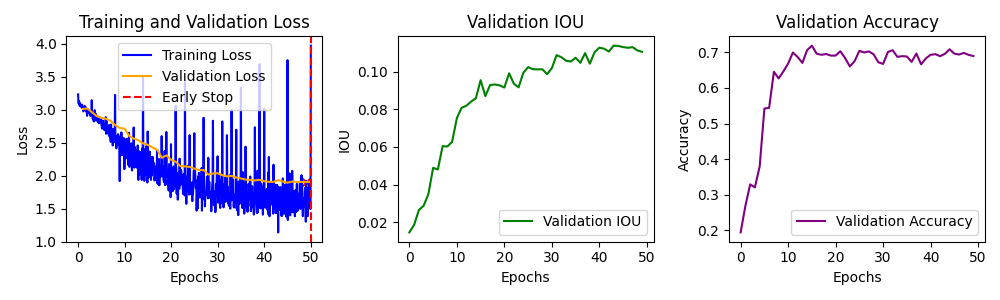
\includegraphics[width=\textwidth]{plots/darrennet_transfer}
	\caption{DarrenNet Transfer}
	\label{fig:darren_transfer}
\end{figure}


Figure \ref{fig:darren_transfer_aug} represents the results of DarrenNet with both transfer learning and data augmentation. This combination appears to be highly effective, as the model achieves impressive segmentation results on the test set. The incorporation of augmented data during training, along with knowledge transfer, contributes to enhanced generalization capabilities.

\begin{figure}[H]
	\centering
	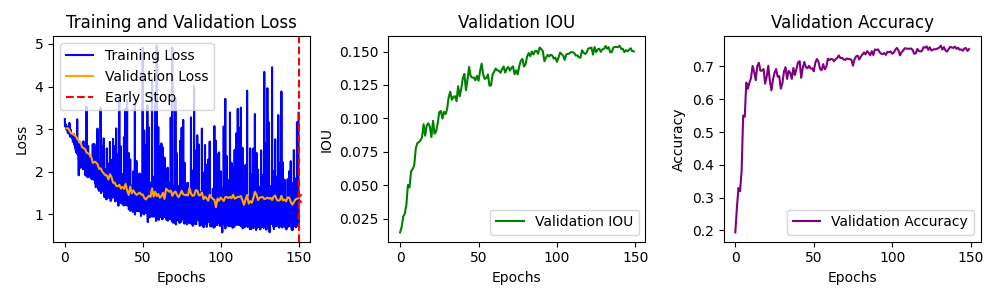
\includegraphics[width=\textwidth]{plots/darrennet_transfer_augment}
	\caption{DarrenNet Transfer Augment}
	\label{fig:darren_transfer_aug}
\end{figure}

Figure \ref{fig:darren_aug_aff} displays the results of the DarrenNet with Augment Affine and transfer learning. Validation set had the following metrics: average IOU of 0.18 and pixel accuracy of 81\%. The model exhibits strong performance on the test set, achieving a high Intersection over Union (IOU) at 0.15 and 82\% accuracy. The augmentation techniques, particularly affine transformations, seem to enhance the model's ability to generalize well to unseen data, resulting in improved segmentation accuracy.

\begin{figure}[H]
	\centering
	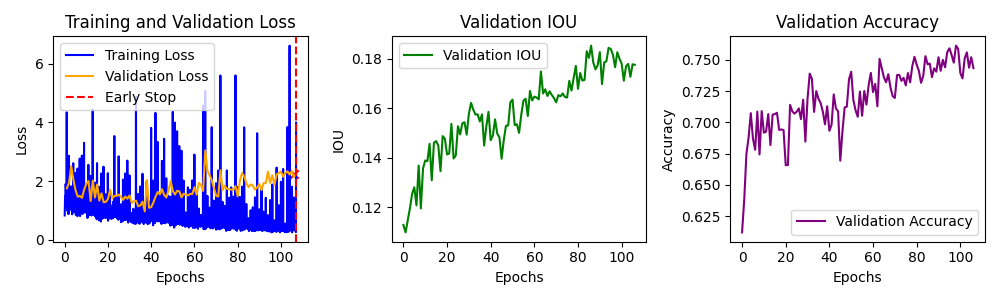
\includegraphics[width=\textwidth]{plots/darrennet_augment_affine}
	\caption{DarrenNet Augment Affine}
	\label{fig:darren_aug_aff}
\end{figure}


The UNet architecture's results are depicted in Figure \ref{fig:unet}. The validation set had an IOU of 0.08 and pixel accuracy of 0.63\% The model demonstrates below average segmentation performance, achieving poor IOU (0.05) and accuracy (0.55) on the test set.

\begin{figure}[H]
	\centering
	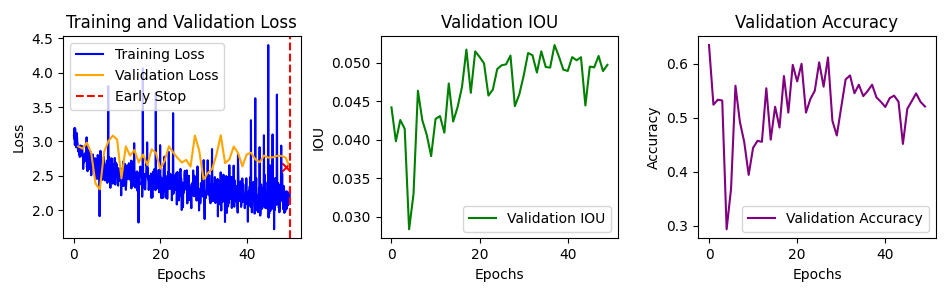
\includegraphics[width=\textwidth]{plots/unet}
	\caption{UNet}
	\label{fig:unet}
\end{figure}

In Figure \ref{fig:unet_transfer}, we observe the UNet with transfer learning. The model exhibits improved segmentation results compared to the non-transfer counterpart, showcasing the effectiveness of leveraging pre-trained weights. The average pixel accuracy and IOU from the validation set were 0.1 and 77\% Transfer learning enhances the model's ability to understand and segment structures in the medical images, leading to higher IOU (0.08) and accuracy (79\%) on the test set.

\begin{figure}[H]
	\centering
	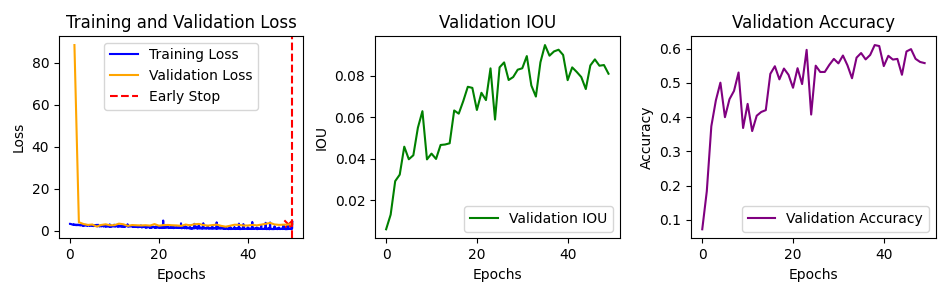
\includegraphics[width=\textwidth]{plots/unet_transfer}
	\caption{UNet Transfer}
	\label{fig:unet_transfer}
\end{figure}


We see the best results with DarrenNet that leverages pretrained ERFNet weights. Unet also
gives decent results, at least when it comes to detecting humans \ref{fig:comparison}.

\begin{figure}[H]
	\centering
	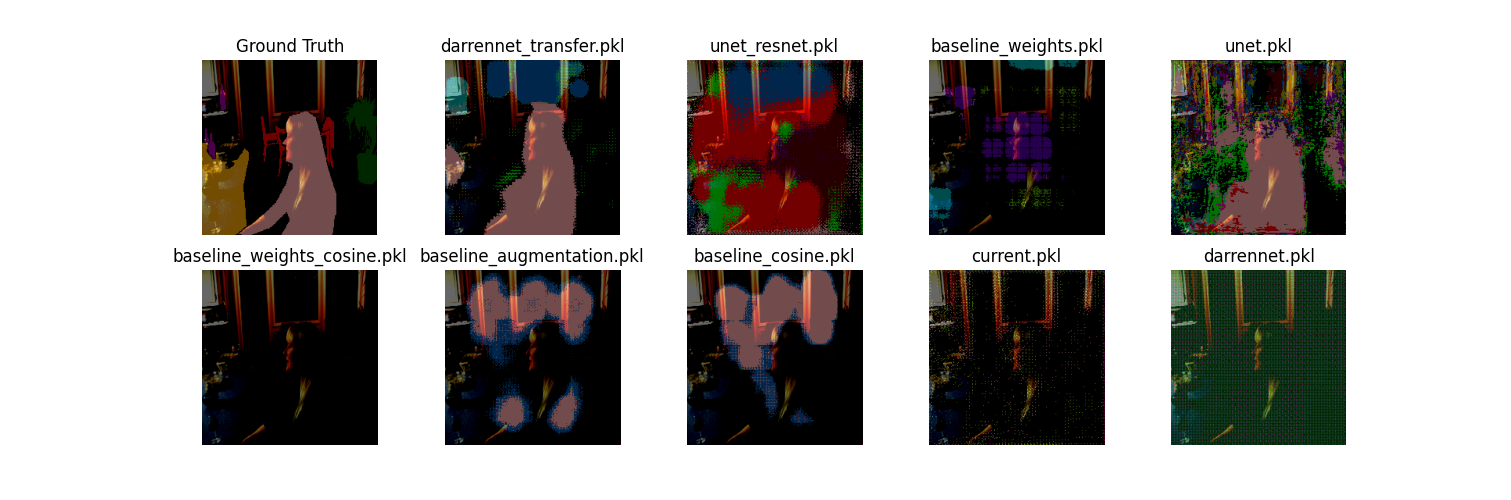
\includegraphics[width=\textwidth]{plots/comparison}
	\caption{Comparison between models}
	\label{fig:comparison}
\end{figure}
